% !TEX root = ../../Tesi_Triennale_PMNS.tex
\chapter[Osservazioni di onde gravtazionali]{Osservazione di onde gravitazionali prodotte da un sistema binario di stelle di neutroni}
\label{chapter:gw170817}
\begin{wrapfigure}{r}{0.4\textwidth}
	\vspace{-10pt}
	\begin{center}
		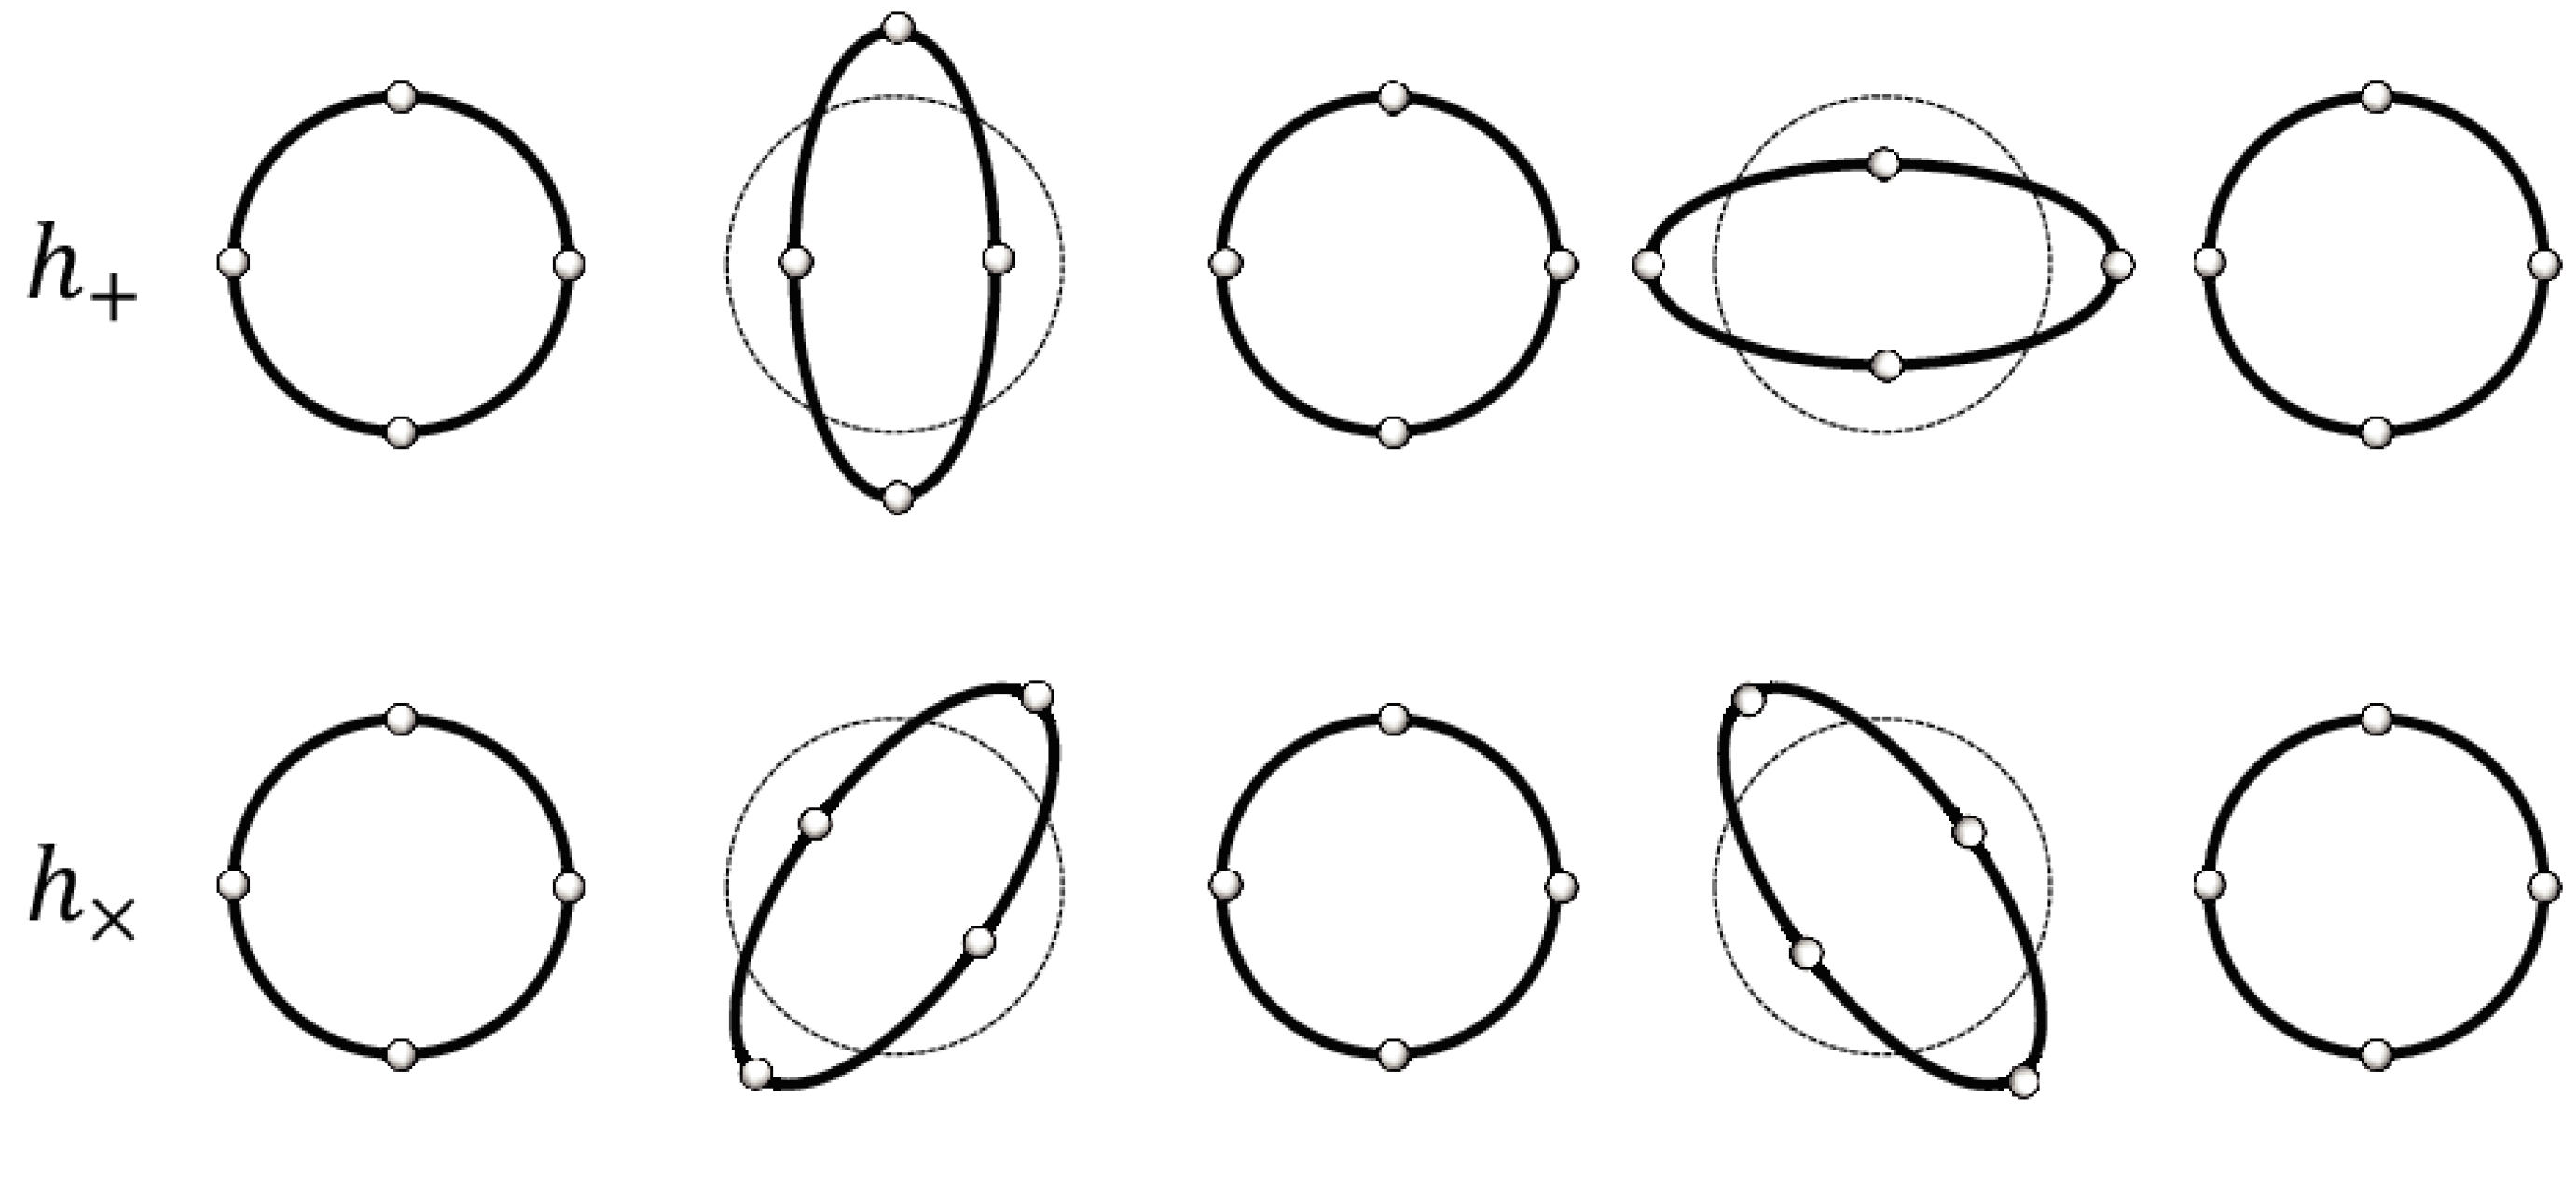
\includegraphics[width=0.4\textwidth]{figures/Capitolo_2/gw_effect.png}
	\end{center}
	\vspace{-5pt}
	\caption{Effetto su un sistema di particelle su piano dovuto al passaggio di un'onda gravitazionale che si propaga ortogonalmente al piano, \cite{universe3030059}}
	\label{fig:gweffect}
	\vspace{-10pt}
\end{wrapfigure}
Gli effetti fisici del passaggio di un'onda gravitazionale si manifestano nell'interazione con le masse, in particolare è necessario considerare sistemi di due o più corpi poiché, in accordo con il principio di equivalenza, è sempre possibile trovare un sistema di riferimento in cui poter applicare le leggi della relatività speciale. Ciò che bisogna considerare è invece l'accelerazione reciproca tra due corpi, in particolare si dimostra che, con il passaggio della GW, la distanza che separa i due corpi subisce periodicamente contrazioni e allungamenti nella direzione della congiungente.
È facile dedurre l'effetto che si osserva per sistemi di particelle sia quello di Figura \ref{fig:gweffect}. Questo effetto può essere usato nella rivelazione, tuttavia non è possibile raggiungere sensibilità sufficienti per le ampiezze estremamente limitate di un'onda gravitazionale. 

Il metodo più usato per la rivelazione è invece quello interferometrico basato sul modello classico dell'interferometro di Michelson: un fascio di luce laser monocromatica viene diviso con l'utilizzo di uno splitter con uguale probabilità di trasmettere o riflettere il fascio, in due bracci tra loro perpendicolari; i due fasci vengono poi riflessi ricombinandosi sullo splitter e venendo raccolti da un fotodiodo che ne misura l'intensità. Il passaggio di un'onda gravitazionale che si muove perpendicolarmente al piano dell'interferometro porta l'allungamento di un braccio e la contrazione dell'altro e quindi a una variazione nella fase tra i due fasci e una variazione della potenza registrata dal fotodiodo.\\
%\begin{wrapfigure}{r}{0.4\textwidth}
%	\vspace{-10pt}
%	\begin{center}
%		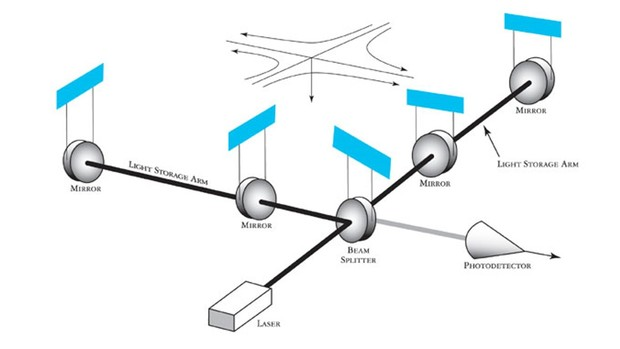
\includegraphics[width=0.4\textwidth]{figures/Capitolo_2/michelson.jpg}
%	\end{center}
%	\vspace{-5pt}
%	\caption{Rappresentazione schematica di un interferometro utilizzato per la rivelazione di segnali di onda gravitazionale}
%	\label{fig:michelson}
%	\vspace{-10pt}
%\end{wrapfigure}
È possibile massimizzare gli effetti del modello classico dell'interferometro di Michelson con tecniche come cavità ottiche, che permettono di avere bracci "efficaci" di lunghezze non ottenibili altrimenti, oltre che tecniche per ridurre il rumore attraverso l'utilizzo di materiali tali da minizzare l'assorbimento del fascio.\\
È possibile inoltre combinare vari rivelatori in una rete per coprire porzioni maggiori del cielo e per verificare la coerenza tra i segnali e poter scartare gli eventi di rumore rivelati dai singoli rivelatori.\\
Il network LIGO-Virgo che si utilizza è composto da tre rivelatori (LIGO-Livingston in Luisiana, LIGO-Hanford in Washington e Virgo in Italia) e nel futuro verrà esteso con l'aggiunta di Kagra in Giappone e LIGO-India in India.
\section{Osservazione della coalescenza di un sistema di stelle di neutroni: GW170817}
\label{section:osservazioneInspiralGW170817}
Rivelato il 17 Agosto 2017 dal network LIGO-Virgo, GW170817 è il primo segnale di onda gravitazionale generato dallo spiraleggiamento di un sistema binario di stelle di neutroni.
Il segnale, osservato alla fine del secondo run di misure O2, è tutt'ora il più energetico osservato tra questi tipi di segnale con un rapporto segnale su rumore (SNR) di 32.4.
Oltre al segnale di GW è stato osservato un lampo-gamma, dopo 1.7s dalla coalescenza.

Il segnale è chiaramente visibile nella rappresentazione tempo-frequenza dei dati in Figura  \ref{fig:osservazione_gw170817}, nei rivelatori LIGO, risulta invece aver un rapporto segnale rumore più basso in Virgo, a causa della minor sensibilità del detector rispetto alla posizione nel cielo della sorgente. La (non) rivelazione risulta comunque utile, soprattutto per permettere l'individuazione della posizione celeste della sorgente.

%Dalla rappresentazione tempo-frequenza dei dati, a cui viene sottratto il rumore e sbiancati, si può notare immediatamente che il segnale che è ben visibile nei due rivelatori LIGO, mentre in Virgo, a causa della posizione celeste della sorgente del segnale, non è possibile distiguere visivamente nessun pattern rispetto rumore di fondo. 
\begin{wrapfigure}{r}{0.4\textwidth}
	\vspace{-25pt}
	\begin{center}
		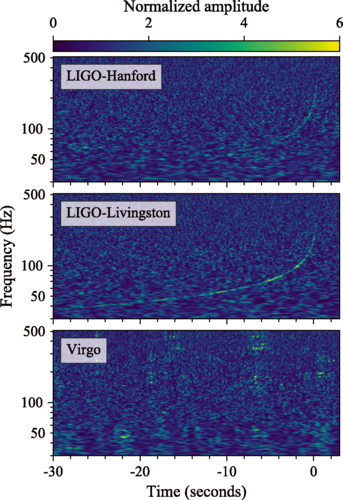
\includegraphics[width=0.4\textwidth]{figures/Capitolo_2/gw170817_time_freq.png}
	\end{center}
	\vspace{-7pt}
	\caption{Segnali nella mappa tempo frequenza nel network, \cite{Abbott_2017a}}
	\label{fig:osservazione_gw170817}
	\vspace{-25pt}
\end{wrapfigure}
L'analisi a bassa latenza dell'evento ha mostrato un segnale coerente nei due detector LIGO, grazie al quale si individua la sorgente in una regione identificata da un angolo solido di 31 $\text{deg}^2$, che a sua volta ha permesso l'identificazione della controparte elettromagnetica GRB170817A. 
Si è ottenuto inoltre un SNR combinato tra i detector di 32.4 che rendono questo segnale il più intenso rivelato finora\cite{Abbott_2017a}.

%La relatività generale fa previsioni abbastanza dettagliate sull'evoluzione della frequenza, che è legata, nella prima fase, a una combinazione delle masse delle stelle progenitrici, detta massa di chirp 
%\begin{equation}
%	\mathcal{M} = \frac{(m_1m_2)^{3/5}}{(m_1+m_2)^{1/5}}
%	\label{eqn:chirpmass}
%\end{equation}
%Nelle fasi più avanzate, le orbite si stringono e aumenta la frequenza dell'onda gravitazionale, mentre la fase della GW è sempre più influenzata da effetti relativistici legati al rapporto tra le masse $q = m_2/m_1$ e dagli accoppiamenti spin-orbita e spin-spin. 
%La composizione interna degli oggetti diventa importante quando la distanza tra essi diventa paragonabile alle dimensioni dell'oggetto stesso. 
Valgono le previsioni sulla frequenza fatte nel Capitolo \ref{chapter:segnaleGWdaBNS} per la prima fase di spiraleggiamento. Nelle fasi più avanzate, le orbite si stringono e aumenta la frequenza dell'onda gravitazionale, mentre la fase della GW è sempre più influenzata da effetti relativistici legati al rapporto tra le masse $q = m_2/m_1$ e dagli accoppiamenti spin-orbita e spin-spin. La composizione interna degli oggetti diventa importante quando la distanza tra essi diventa paragonabile alle dimensioni dell'oggetto stesso. 

Le proprietà della sorgente di onde gravitazionali sono ottenute dal confronto con le forme d'onda predette dalla teoria. Viene fatta dunque una analisi Bayesiana nel range di frequenze 30-2048Hz che include gli effetti dell'incertezza di calibrazione di $1\sigma$ sul segnale ricevuto.\\Per la stima del rumore, le fonti risultano molteplici e data la difficoltà nello stimare il rumore in assenza di sorgenti, non potendo "spegnere" le fonti di onde gravitazionali, la stima viene fatta a partire dai dati di una sessione di misure limitata, che però viene riprodotta e traslata temporalmente tra un rivelatore e l'altro in modo da annullare eventuali coerenze tra i segnali rivelati. Con questa operazione si può ottenere un fondo di migliaia di anni a partire dai dati di pochi giorni.

\begin{wrapfigure}{r}{0.4\textwidth}
	\vspace{-22pt}
	\begin{center}
		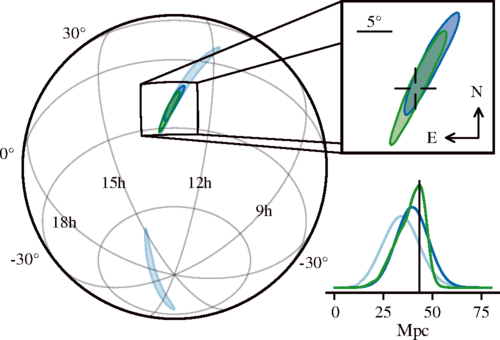
\includegraphics[width=0.4\textwidth]{figures/Capitolo_2/skymap.png}
	\end{center}
	\vspace{-5pt}
	\caption{Sky location ricostruita per GW170817, nella versione preliminare in blu chiaro per Hanford-Livingston e in blu scuro per Handord-Livingston-Virgo, mentre nella versione finale in verde, presa da \cite{Abbott_2019}}
	\label{fig:skymap}
	\vspace{-20pt}
\end{wrapfigure}
Attraverso un'analisi più approfondita dei dati consolidati, la sorgente viene identificata in una regione celeste di 28$\text{deg}^2$ di area e $380\text{Mpc}^3$ di volume, utilizzando una combinazione di timing, fase e ampiezza dei tre detector. La distanza luminosa, la più prossima osservata finora, viene individuata in $40_{-14}^{+8}$Mpc. La massa di chirp del sistema si valuta in $\mathcal{M}=1.188_{-0.002}^{+0.004}$, mentre la valutazione delle masse delle stelle progenitrici dipende dalla prior scelta per l'analisi, legata alla scelta dell'EOS che si considera, si stimano dunque interavalli $m_1 \in (1.36, 2.26)M_\odot$ e $m_2 \in (0.86, 1.36)M_\odot$, che, nonostante la grande imprecisione, costituiscono un'evidenza della natura di stelle di neutroni del sistema binario, escludendo invece la possibilità di buchi neri che prevederebbe range di masse superiori\cite{Abbott_2017a}.
%Per le masse delle stelle compatte risulta più semplice dedurre la massa di chirp, indipendente dalla scelta della prior nell'analisi Bayesiana legata all'equazione di stato scelta per le stelle progenitrici, che si valuta in $\mathcal{M}=1.188_{-0.002}^{+0.004}$, rispetto alle masse singole, che soffrono invece della degenerazione tra il rapporto tra le masse $q$ e le componenti dello spin $\chi_1$ e $\chi_2$. È necessario fare quindi assunzioni a partire dalle EOS che si considerano, ottenendo dei range $m_1 \in (1.36, 2.26)M_\odot$ e $m_2 \in (0.86, 1.36)M_\odot$ evidentemente meno precisi, ma comunque utili come evidenza della natura di stelle di neutroni del sistema binario, escludendo invece la possibilità di buchi neri che prevederebbe range di masse superiori\cite{Abbott_2017a}.

Oltre al segnale di onda gravitazionale è stato rivelato anche un segnale di short gamma-ray burst dal telescopio spaziale Fermi-GBM, $1.74\pm0.05$s dopo l'istante di coalescenza e della durata di circa 2 secondi. Il segnale viene rivelato anche dal telescopio INTEGRAL e la differenza dei tempi di arrivo del segnale sui due telescopi ha permesso di migliorare significativamente l'area di localizzazione del segnale.\\
In seguito all'osservazione e alla localizzazione del segnale, diversi telescopi, terrestri e spaziali, vengono direzionati in modo tale da poter osservare il corpo celeste formatosi: la prima osservazione viene fatta dai telescopi dell'osservatorio di Las Campas in Cile circa 10h dopo la coalescenza. Osservando le galassie conosciute viene individuato un unico evento transiente, non corrispondente ad alcun asteroide o supernova conosciute. Dopo la prima osservazione, altri 5 team registrano l'evento. Queste localizzazioni sono state importanti per identificare con maggior precisione la distanza alla quale è avvenuto l'evento\cite{Abbott_2017c}.
%QUALCOSA SULLE TIDAL DEFORMABILITIES?
\section{Ricerca del post-merger del residuo}
\label{section:postmergerGW170817}
È stata effettuata un'analisi specifica per ricercare un eventuale segnale nella fase di post-coalescenza, tuttavia tale analisi non ha portato ad evidenza statisticamente significativa di rivelazione di un segnale nella fase di coalescenza, ma ha permesso di ottenere informazioni sul limite superiore delle ampiezze di strain ed energie di GW osservabili. Gli attuali detector infatti non hanno una sensibilità tale da permettere rivelazioni alle alte frequenze della post-coalescenza.

Per la ricerca di segnali con incertezze teoriche così grandi risulta inefficiente l'utilizzo di metodi di ricerca matched-filtering, ovvero metodi che utilizzano segnali di forme conosciute e, attraverso funzioni di filtraggio escludono la componente di rumore, usando come filtro la funzione che massimizza il rapporto segnale su rumore (SNR) per tale segnale\cite{maggiore2008gravitational}. È immediato comprendere che non conoscendo con certezza la forma che deve assumere il segnale questo metodo risulta inefficace per la ricerca del post-merger. Gli algoritmi che si usano invece ricercano eccessi di potenza in una mappa tempo-frequenza e, usando metodi di riconoscimento dei pattern, possono identificare la presenza di segnali di GW. In particolare gli algoritmi sono tali da considerare i dati della rete e non dei singoli rivelatori, utilizzando tecniche che permettono di combinare coerentemente i dati dei singoli rivelatori e dare risposte differenti a forme d'onda diverse.

Mentre lo studio del segnale elettromagnetico associato alla GW non permette di escludere nessuno dei possibili stati finali indicati in sezione \ref{section:residual}, grazie ai valori ottenuti per le masse dei progenitori date nella sezione \ref{section:osservazioneInspiralGW170817} si calcola che per un ampio range di equazioni di stato la coalescenza produce uno stato di NS ipermassiva. Questo spiega anche il ritardo del lampo gamma rispetto all'istante di rivelazione del segnale di merger. 

Come si vedrà nella sezione \ref{section:examples} in base alla EOS che si considera si ottiene un contributo diverso nel post-merger che inizia attorno a $\smallsim2$kHz. Più in generale, oltre alla EOS hanno fondamentale importanza le masse e gli spin degli oggetti iniziali. 
Per quanto riguarda invece la rivelazione di questa fase del segnale, anche considerando modelli ottimistici da stati finali di NS ipermassiva o supermassiva, l'SNR atteso per distanze di $\smallsim40$Mpc è $\smallsim1-2$ ordini di grandezza più piccolo di quello rivelabile dalla rete LIGO-Virgo attualmente utilizzata, facendo uso di algoritmi di confronto con segnali modellati (che comunque sono meno utilizzati per la post-coalescenza per i motivi già citati).
Si ipotizza tuttavia che nei prossimi run la sensibilità del network sarà tale da permettere la rivelazione di queste emissioni\cite{Abbott_2017b}, e si studierà nel dettaglio nel Capitolo \ref{chapter:analisi}.

\begin{wrapfigure}{r}{0.5\textwidth}
	\vspace{-20pt}
	\begin{center}
		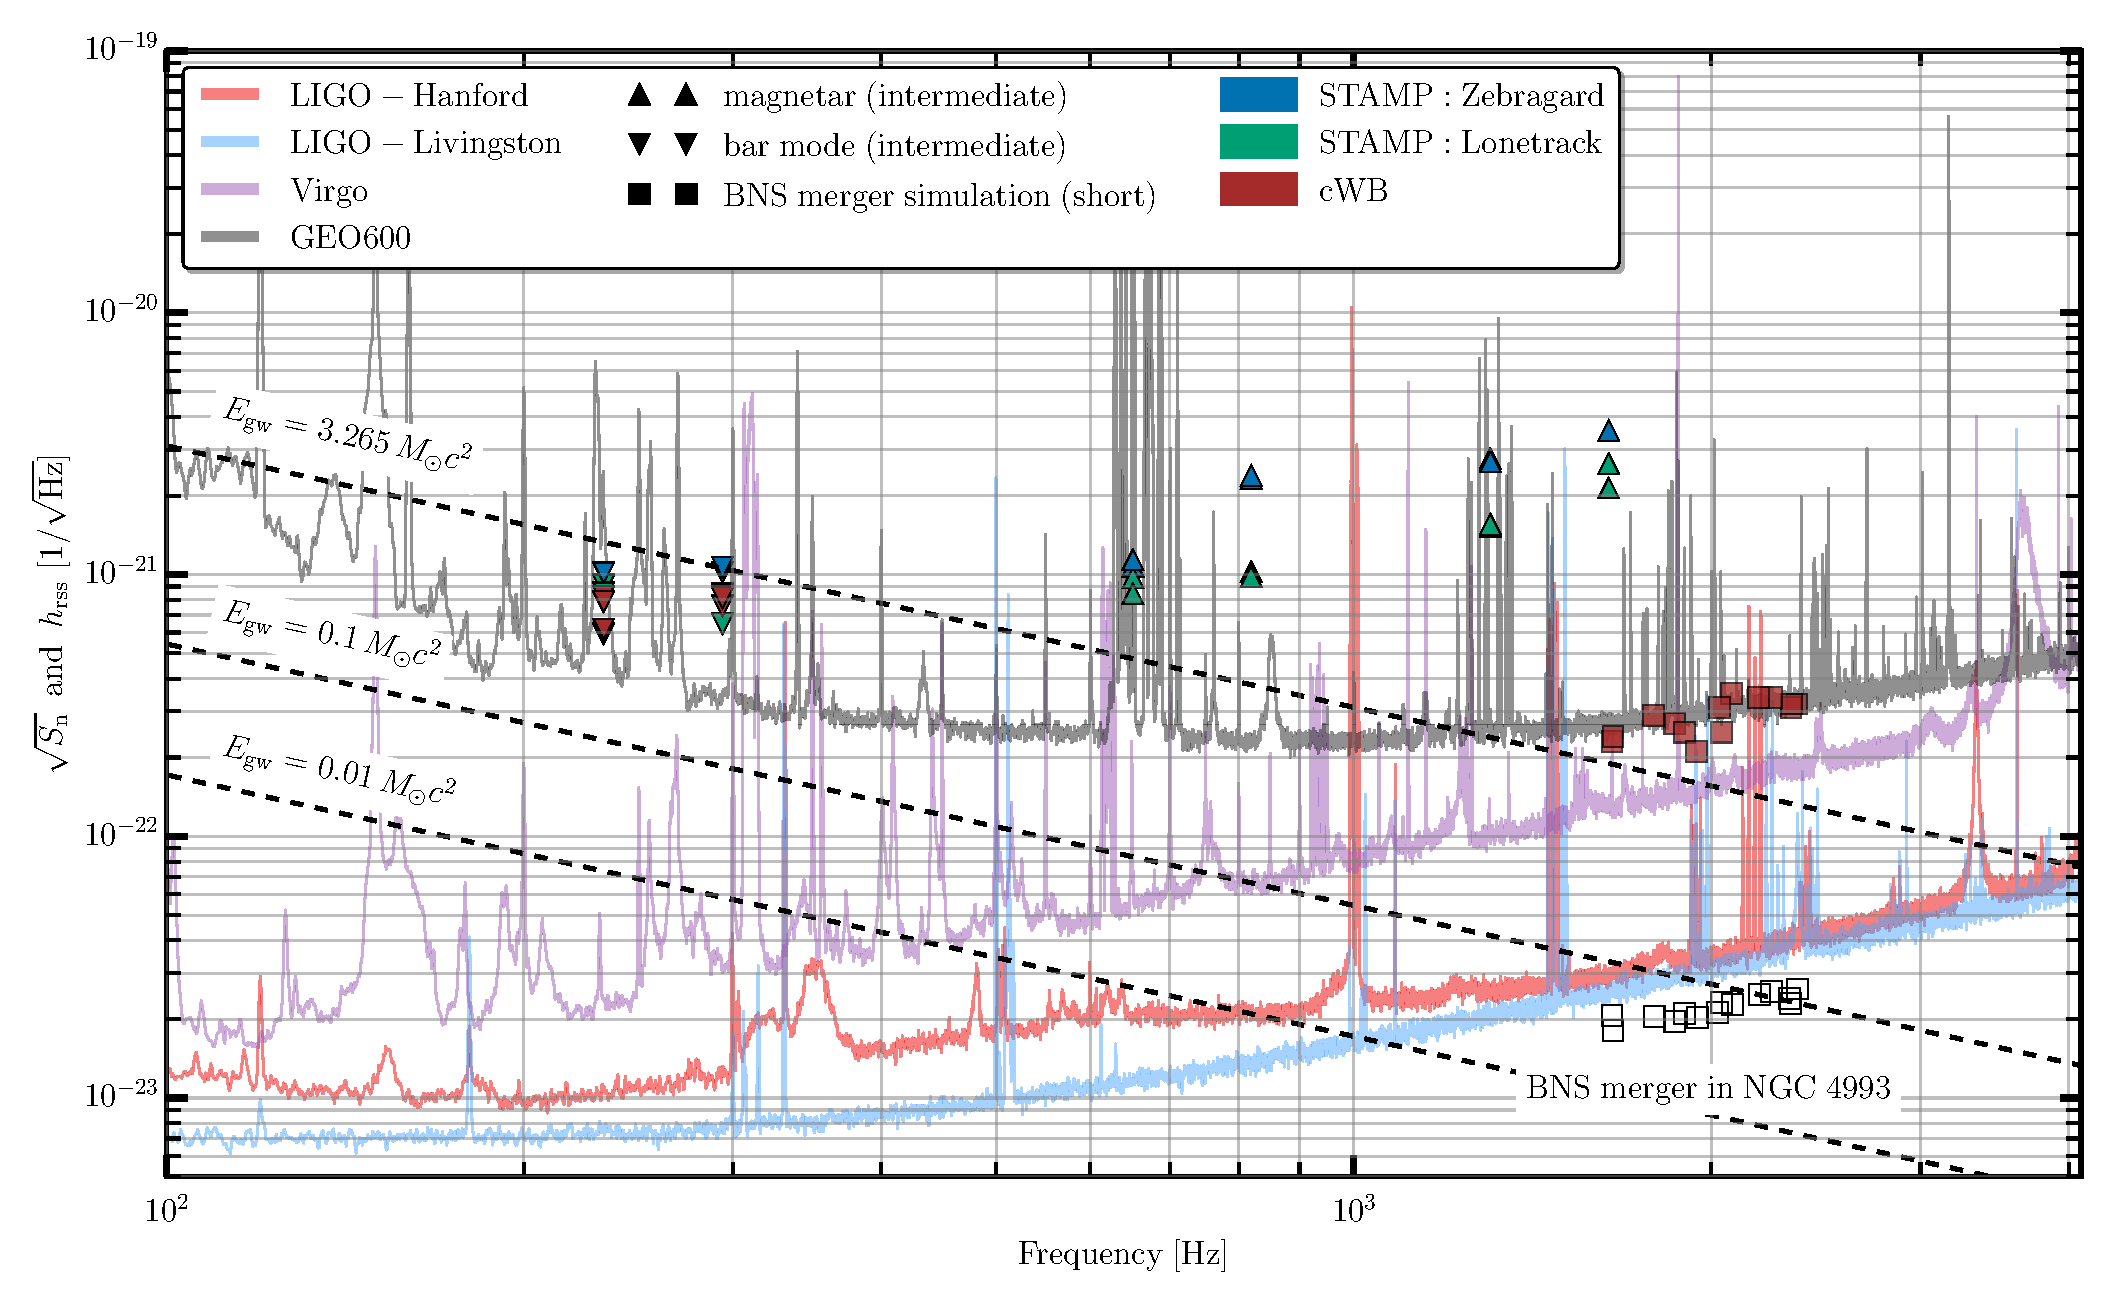
\includegraphics[width=0.5\textwidth]{figures/Capitolo_2/GW170817_spectral_limits.pdf}
	\end{center}
	\vspace{-5pt}
	\caption{Sensibilità di ciascun rivelatore durante il run O2, indicata dall'ampiezza del rumore di strain in funzione della frequenza, \cite{Abbott_2017b}}
	\label{fig:NoiseFrequenze}
	\vspace{-10pt}
\end{wrapfigure}
Come si può osservare in Figura \ref{fig:NoiseFrequenze} i tre detector del network hanno zone diverse di sensibilità al segnale considerato, in particolare si nota che in generale la sensibilità diminuisce significativamente ad alte frequenze. 

La ricerca è stata effettuata utilizzando diversi algoritmi, e su diversi range di frequenza. È stato utilizzato l'algoritmo cWB, per la ricerca di segnali di breve durata (fino ai pochi secondi), nel range di frequenza 1024-4096 Hz. 
Un'ulteriore ricerca è stata effettuata per cercare segnali di più lunga durata (dalla decina alle poche centinaia di secondi) utilizzando l'algoritmo cWB nella banda di frequenza 24-2048Hz, e STAMP nella banda 24-4000Hz.

%Per l'analisi sono stati usati due diversi algoritmi, in base al tipo di segnale ricercato: per segnali di brave durata è stato usato cWB (Coherent Wave Burst) utilizzando i dati di LIGO tra 1024Hz e 4096Hz, mentre per i segnali di durata intermedia si è utilizzato l'algoritmo STAMP (Stochastic Transient Analysis Multidetector Pipeline) nelle frequenze comprese tra 24Hz e 2000Hz e tra 2000Hz e 4000Hz nei dati di LIGO, mentre cWB con i dati del network LIGO-Virgo ricerca le frequenze tra 24Hz e 2048Hz.
%Come anticipato, la ricerca viene divisa tra segnali brevi ($\lesssim$1s) e intermedi ($\lesssim$500s).
%\subsection{Segnali brevi}
L'analisi dei segnali brevi ad alte frequenze consiste nella ricerca di eccessi di potenza nell'intervallo di 2s che precede il segnale elettromagnetico GRB 170817a, in un intervallo che comprende quindi anche la coalescenza.

%In particolare l'algoritmo valuta la massima verosimiglianza di eccessi di potenza in una trasformata di wavelet a multi-risoluzione per ogni detector, classificando gli eventi in una gerarchia di SNR. La significanza degli eventi è data dal confronto con la distribuzione del fondo stocastico, che è generata con metodi che saranno precisati nel capitolo \ref{chapter:cwb}. 
È convenzione esprimere la sensibilità della ricerca di una data forma d'onda in $h_{rss}^{50\%}$, ovvero la somma in quadratura delle ampiezze di strain di segnali che sono rivelati con un'efficienza del 50\%. La quantità $h_{rss}$ è definita come
\begin{equation}
	h_{rss} = \sqrt{2\int_{f_{min}}^{f_{max}}df(|\tilde{h}_+(f)|^2 + |\tilde{h}_\times(f)|^2 )}
\end{equation}
dove $f_{min}$ e $f_{max}$ sono rispettivamente le frequenze massima e minima sulle quali si effettua la ricerca. 
Il criterio sulla soglia di rivelazione e quindi su $h_{rss}^{50\%}$ per questo metodo di ricerca è tale da garantire una probabilità di falso allarme di $10^{-4}$.
Per evitare la possibile perdita di segnali di EOS rigide, la ricerca viene effettuata a partire da 1024Hz, nonostante le previsioni teoriche mostrino una frequenza sempre maggiore.
%a frequenza maggiore si fa la scelta conservativa di ricercare segnali a partire da 1024Hz, nonostante tutte le forme d'onda abbiano emissioni dominanti molto al di sopra di tale soglia.

In conclusione, non viene trovata evidenza di nessun segnale di GW in questa banda di frequenze.
L'ampiezza di strain per produrre una probabilità del 50\% di rivelazione di un segnale è compresa tra $2.1 \times 10^{-22} \text{Hz}^{-1/2}$ e $3.5 \times 10^{-22} \text{Hz}^{-1/2}$. L'energia irradiata da un sorgente che emette isotropicamente è data da 
\begin{equation}
	E_{gw}^{iso} = \frac{\pi c^3}{2G}\mathcal{D}^2\int d\Omega \int_{f_{min}}^{f_{max}}dff^2(|\tilde{h}_+(f)|^2 + |\tilde{h}_\times(f)|^2 ) \approx \frac{\pi^2 c^3}{G}\mathcal{D}^2\bar{f}^2h_{rss}^2
\end{equation}
con $\mathcal{D}$ è la distanza dalla sorgente e $\bar{f}$ è la frequenza caratteristica data da 
\begin{equation}
	\bar{f} = \frac{2}{h_{rss}^2}\int_{f_{min}}^{f_{max}}dff(|\tilde{h}_+(f)|^2 + |\tilde{h}_\times(f)|^2 )
\end{equation}
In questo modo si ottiene un range di energie rivelabili che, secondo il criterio del $h_{rss}^{500\%}$, è dato da $4.8-\SI{19.6}{\solarmass}c^2$, al di fuori delle masse in gioco per BNS, per cui non è possibile con i rivelatori attuali rivelare le emissioni di GW di NS ipermassive associate a GW170817.
%\subsection{Segnali di durata intermedia}

Per segnali di durata intermedia si utilizzano i due algoritmi cWB e STAMP, concentrando la ricerca in una zona limitata dello spazio, indicata dalla controparte elettromagnetica che permette di evitare trigger accidentali.\\
%Sono considerate due morfologie di forme d'onda corrispondenti a GW da bar-modes secolari o causati da elicità causate dal campo magnetico nella stella nascente. I meccanismi di emissione attraverso modi-r non sono considerati per la durata che richiederebbe scale temporali più lunghe.
\\
%Nell'analisi di STAMP, che ricerca segnali in uno spettrogramma con pixel di 1s$\times$1Hz, creati con la correlazione incrociata dei dati di detector spazialmente separati, sia con metodi seed-based clustering, dove per seed si intendono pixel con un eccesso di potenza sopra una certa soglia che vengono connessi formando un cluster, sia con algoritmi seedless, senza quindi applicare soglie minime, per il riconoscimento dei pattern, non viene trovato nessun significativo eccesso di potenza, con una probabilità di falso allarme di $10^{-2}$.
Mentre l'analisi fatta con l'algoritmo STAMP non viene qui approfondita, l'analisi con cWB è analoga alla precedente, ma considera un intervallo di tempo che parte dal merger e copre 1000s. Per entrambe le analisi, con probabilità di falso allarme di $10^{-2}$ per STAMP e di $10^{-4}$ per cWB, nessun candidato è trovato nella banda di frequenza considerata. È possibile confrontare il range di energie rivelabili in Figura \ref{fig:NoiseFrequenze}.

Concludendo, non viene trovata nessuna evidenza di un segnale di post coalescenza nei dati considerati: se esiste un segnale questo è comunque troppo debole per essere rivelato dai rivelatori nel run O2 \cite{Abbott_2017b}.

\section{Segnale GW190425}
%\subsection*{GW190425}
Il secondo evento rivelato di spiraleggiamento di BNS è GW190425 durante il run O3 del network Virgo-LIGO. In realtà durante l'evento il detector LIGO Hanford era spento, quindi il network contava solo su due rivelatori. Non sono inoltre stati rivelati segnali elettromagnetici associati all'evento.\\
L'evento ha avuto un SNR di 12.9 per LIGO Livingston mentre di solo 2.5, ovvero sotto la soglia di trigger pari a 4, per Virgo. La differenza tra i due rivelatori è consistente con la differenza di sensibilità tra i due detector\cite{Abbott_2020b}.

%\paragraph{Proprietà della sorgente} 
In continuità con le definizioni fatte per le proprietà del segnale GW170817, si riportano brevemente le caratteristiche del segnale GW190425: si individua la sorgente in un'area celeste di 8284deg$^2$ al 90\% di credibilità (estremamente più impreciso di GW170817) e la distanza viene valutata in $159_{-71}^{+69}$Mpc. La così più grande incertezza rispetto al primo segnale è dovuta al minor numero di detector coinvolti e all'impossibilità di escludere regioni grazie alla controparte elettromagnetica che non viene rivelata in questo caso.
La massa di chirp è pari a $1.4873^{+0.0008}_{-0.0006}M_\odot$, mentre le masse delle stelle progenitrici sono $m_1 \in (1.60, 2.52)M_\odot$ e $m_2 \in (1.46, 1.68)M_\odot$\cite{Abbott_2020b}.

È stata effettuata anche una ricerca di un eventuale segnale di post-coalescenza, supponendo che il sistema non collassi immediatamente in buco nero. La ricerca, effettuata con metodi alternativi a quelli che verranno descritti nel capitolo \ref{chapter:cwb}, non porta a nessuna evidenza statisticamente significativa di un segnale.
%\begin{wrapfigure}{r}{0.5\textwidth}
%	\vspace{-5pt}
%	\begin{center}
%		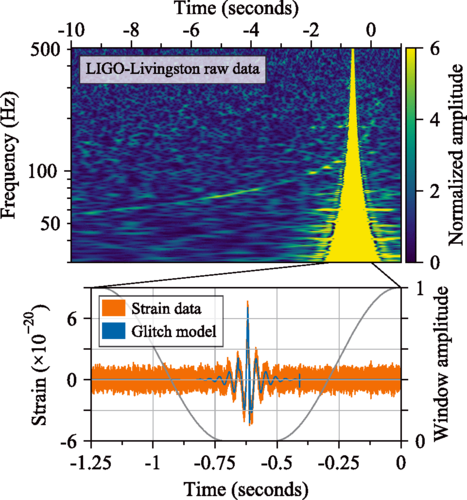
\includegraphics[width=0.5\textwidth]{figures/Capitolo_2/signal.png}
%	\end{center}
%	\vspace{-5pt}
%	\caption{\cite{Abbott_2017b}}
%	\label{fig:signalInspiral}
%	\vspace{-10pt}
%\end{wrapfigure}